\chapter{Diseño Global del Sistema}\label{cap.diseno}

En este capítulo se hace una descripción del diseño global del sistema para llevar a cabo la monitorización de vehículos.

\section{Diseño}

Smart-Traffic-Sensor es un sistema que se realizó con el objetivo de monitorizar tráfico en tiempo real. Es decir para detectar, clasificar y hacer el seguimiento(tracking) de los diferentes vehículos que circulen por la carretera. Los diferentes vehículos que detectemos los clasificaremos en función a 7 clases: car, motorcycle, van, bus, truck, small-truck y tank-truck. 

Actualmente se ha extendido mucho el uso de Deep Learning para la detección y clasificación de objetos, pues con ello se está llegando a obtener muy buenos resultados. Este trabajo se ha basado principalmente en el uso de Deep Learning para la clasificación y detección de vehículos. Además se ha apoyado en \acrshort{klt}, en los casos que pudiera haber pérdidas en la detección debido a oclusiones o cuando los vehículos se encontraban muy alejados. Es decir, se ha apoyado en \acrshort{klt} cuando las condiciones a la hora de detectar eran algo complejas y por tanto el Deep Lerning no era capaz de realizar correctamente la detección.

A la hora de realizar el tracking se hace uso de la distancia euclidea, pero esto se explicará con más detalle en las siguientes secciones.

En resumen se puede decir que tenemos dos grandes bloques:
\begin{itemize}
    \item Detección y Clasificación de vehículos
    \item Tracking de vehículos
\end{itemize}


\section{Bases de Datos de Videos}

La detección de vehículos pretende encontrar un vehículo en una imagen o en un vídeo y determinar qué tipo de
vehículo es. Dado que queremos encontrar el vehículo en cuestión bajo diferentes circunstancias, es decir, en diferentes
entornos y diferentes iluminaciones, necesitaremos entrenar el modelo con un conjunto de imágenes representativo. Por
este motivo, a lo largo de los últimos años han surgido diferentes datasets con el fin de solucionar este problema. Para el caso de la detección de vehículos hay que decir que hay pocos datasets, por ello ha sido necesario crear una base de datos propia.

Esta base de datos propia consta de:
\begin{itemize}
    \item La base de datos empleada por Redouane Kachach~\cite{traffic_monitor_lab}.
    \item La base de datos \acrfull{gram} creada por R. Guerrero-Gomez-Olmedo, R. J. Lopez-Sastre, S. Maldonado-Bascon and A. Fernandez-Caballero~\cite{guerrero2013iwinac} 
    \item Imágenes recopiladas de cámaras en abierto de forma online.
\end{itemize} 

Se ha tratado que la base de datos construida abarcará la mayor diversidad de vehículos posibles y en diferente tipos de escenarios. Hay que tener en cuenta que toda la base de datos tiene vehículos vistos por la parte trasera. En total consta de 9774 imágenes y está formada por 7 clases:
\begin{itemize}
    \item Car
    \item Motorcycle
    \item Van
    \item Bus
    \item Truck
    \item Small-truck
    \item Tank-truck
\end{itemize}

En estas 9774 imágenes tenemos un total de 48914 muestras repartidas tal y como se muestra en la Tabla ~\ref{tabla_muestras}.

\begin{table}[htbp]
\begin{center}
\begin{tabular}{|l|l|}
\hline
Clases & Muestras \\
\hline \hline
Car & 38976 \\ \hline
Motorcycle & 1886 \\ \hline
Van & 5631 \\ \hline
Bus & 401 \\ \hline
Truck & 963 \\ \hline
Small-Truck & 938 \\ \hline
Tank-Truck & 119 \\ \hline
\end{tabular}
\caption{Muestras de la Base de Datos}
\label{tabla_muestras}
\end{center}
\end{table}

Para intentar conseguir un sistema robusto antes diferentes condiciones se ha creado una base de datos que tiene imágenes en condiciones meteorológicas buenas, imágenes en condiciones meteorológicas malas (con niebla y lluvia) e imágenes de mala calidad. En la Tabla ~\ref{tabla_img_base_datos} se pueden ver la cantidad de imágenes que hay para cada tipo.
\begin{table}[htb]
\begin{center}
\begin{tabular}{|l|l|}
\hline
\cline{2-2}& Nº de Imágenes\\
\hline \hline
Buena calidad & 8406 \\ \hline
Malas Condiciones Meteorológicas & 663\\ \hline
Mala Calidad & 705\\ \hline
\end{tabular}
\caption{Imágenes de la Base de Datos}
\label{tabla_img_base_datos}
\end{center}
\end{table}

\section{Calibración de la Cámara}


\section{Funcionamiento General}

En esta sección se explica en que técnicas se basa la aplicación Smart-Traffic-Sensor en cuanto a la detección, clasificación y el seguimiento de vehículos.

\subsection{Detección y Clasificación de Vehículos}

En este punto se va a explicar como se ha abordado el problema de la detección y clasificación de vehículos.

Tal y como ya se ha comentado anteriormente se ha hecho uso de Deep Learning. En concreto se ha diseñado un sistema capaz de soportar redes neuronales entrenadas con diferentes frameworks (TensorFlow, Darknet y Keras) con el objetivo de detectar y clasificar los diferentes vehículos que aparezcan en la imagen.

Se han probado tres frameworks diferentes para evaluar cual era el que mejores resultados obtenía. Para ello se hizo un primer entrenamiento con imágenes únicamente de buena calidad con el fin de determinar cual era el framework que mejor funcionaba.

En los siguientes puntos se va a explicar el diseño que se ha llevado a cabo con cada framework, asi como el diseño final empleado en Smart-Traffic-Sensor.

\subsubsection{TensorFlow}

Para llevar a cabo el diseño se ha hecho uso del github models de TensorFlow ~\cite{tensorflow_models}, con el cual podemos entrenar una red pe-entrenada con nuestra propia base de datos. En este caso se ha empleado una red \acrfull{ssd} Mobilenet V2 entrenada con \acrshort{coco}, pues proporciona una buena relación entre la velocidad y la precisión. Para emplear dicha red se ha usado un archivo de configuración llamado ssd\_mobilenet\_v2\_coco.config~\cite{ssd_mobilenetv2_config}.

La red \acrshort{ssd} MobileNet V2 es una red \acrshort{ssd} que en lugar de tener una red VGG-16 de base, tiene una red MobileNet. En la Figura ~\ref{fig.ssd_mobilenet} se puede ver dicho diseño.

\begin{figure}
\begin{center}
	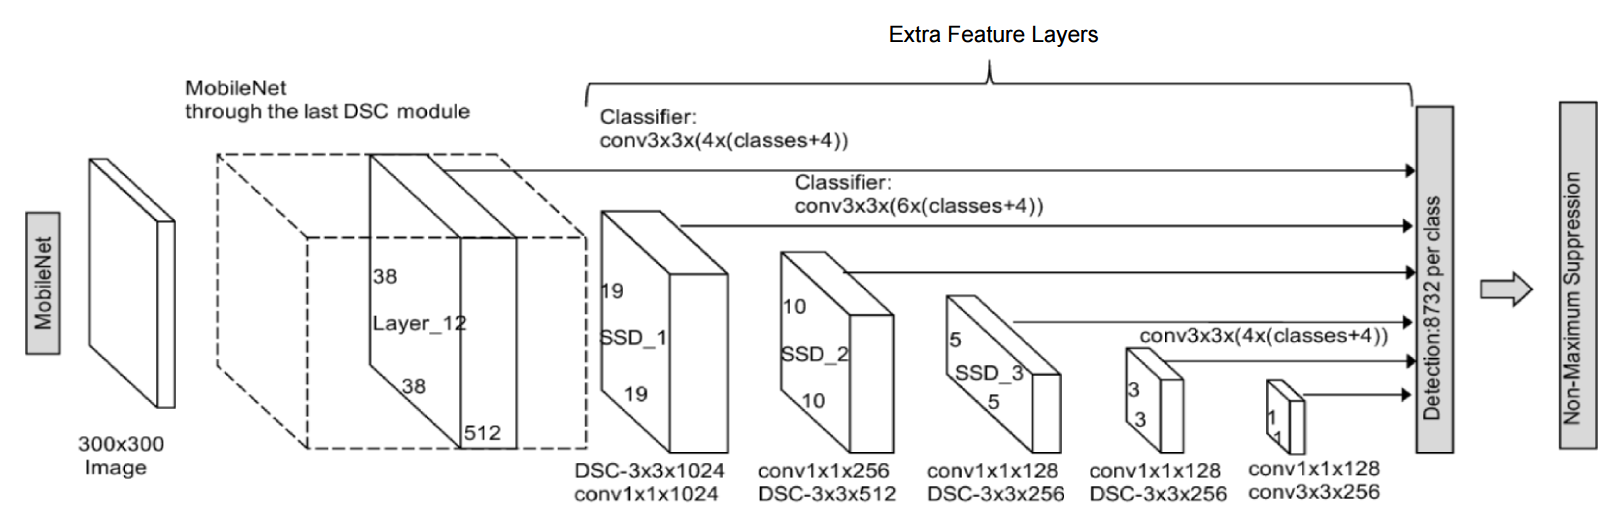
\includegraphics[width=1\textwidth]{figures/Diseno_global/ssd_mobilenet.png}
   \caption{Red SSD Mobilenet V2}
	\label{fig.ssd_mobilenet}
\end{center}
\end{figure}

La primera parte de la red es la Mobilenet V2, en la cual se obtienen los mapas de características para poder realizar la clasificación y detección en las capas posteriores. 

\acrshort{ssd} ~\cite{ssd_article} es un método de detección de objetos en imágenes empleando una única red neuronal profunda. \acrshort{ssd} proporciona una gran ganancia de velocidad frente a Faster \acrshort{rcnn} \cite{rcnn_faster}, que funciona a una tasa de 7 frames por segundo.

El enfoque de \acrshort{ssd} se basa en una red convolucional \textit{feed-forward} que produce un conjunto \textit{bounding boxes} de tamaño fijo y puntúa la presencia de instancias de clase de objeto en esos \textit{bounding boxes}. Tras esto se realiza \textit{non-maximum suppression} para producir las detecciones finales. 

Dada una imagen de entrada y un conjunto de etiquetas de \textit{ground truth}, \acrshort{ssd} realiza el siguiente proceso:
\begin{enumerate}
\item La imagen pasa a través de una serie de capas convolucionales, produciendo varios conjuntos de mapas de características a diferentes escalas.
\item Para cada ubicación en cada uno de estos mapas de características, emplea un filtro convolucional de 3x3 para evaluar un pequeño conjunto de \textit{bounding boxes} por defecto.
\item Para cada \textit{bounding box} predice simultáneamente el desplazamiento del \textit{bounding box} y las probabilidades de clase.
\item Durante el entrenamiento, hace que coincida el \textit{bounding box} del \textit{ground truth} con los \textit{bounding boxes} predichos según IoU (\textit{Intersection over Union}). El mejor \textit{bounding box} predicho se etiquetará como "positivo", junto con todos los demás \textit{bounding boxes} que tengan un ratio de \textit{Intersection over Union} con el \textit{ground truth} mayor de 0.5.
\end{enumerate}

\acrshort{ssd} parece sencillo, pero el entrenamiento tiene un desafío único. Clasificamos y estimamos \textit{bounding boxes} desde cada posición en la imagen, usando múltiples formas diferentes, en diferentes escalas. Como resultado, generamos un número mucho mayor de \textit{bounding boxes} que en otros modelos, y casi todos ellos son ejemplos negativos. Esto introduce un desequilibrio significativo entre los ejemplos de entrenamiento positivos y negativos.

Para solucionar este desequilibrio, SSD hace dos cosas. En primer lugar, utiliza la \acrfull{nms} para agrupar \textit{bounding boxes} muy superpuestos en un solo \textit{bounding box}. En otras palabras, si cuatro \textit{bounding boxes} de formas, tamaños, etc. similares contienen el mismo perro, el \acrshort{nms} conservará el que tenga la mayor confianza y descartará el resto. En segundo lugar, el modelo usa una técnica llamada minería negativa para equilibrar las clases durante el entrenamiento. En la minería negativa dura, solo se utiliza un subconjunto de los ejemplos negativos con la mayor pérdida de entrenamiento (es decir, falsos positivos) en cada iteración de entrenamiento. \acrshort{ssd} mantiene una relación de 3: 1 de negativos a positivos.


La red Mobilenet se basa en la clasificación. Mobilenet emplea unas capas llamadas \textit{depthwise separable cnvolutions} en lugar de capas convolucionales. Las capas textit{depthwise separable cnvolutions} se componen de dos operaciones: \textit{depthwise convolution} y \textit{pointwise convolution}. En una capa convolucional se usan kernels que recorren toda la imagen con el objetivo de extraer información. Estos kernels necesitan tener la misma profundidad que la imagen para ser aplicados, es decir, si tenemos una imagen RGB necesitaremos 3 kernels, uno por cada canal de color. Finalmente estos kernel se combinan para obtener una única imagen. 

En las capas \textit{depthwise separable convolutions} se lleva a cabo el siguiente proceso:
\begin{enumerate}
    \item Se realiza la operación de \textit{depthwise convolution}, en la cual se aplican kernels de igual profundidad que la imagen. Cada kernel se emplea en cada canal de color por separado.
    \item Se lleva a cabo la operación \textit{pointwise convolution} en la cual se aplica un kernel de 1x1xprofundidad de la imagen, con lo que se obtendrá así un único canal.
\end{enumerate}

Si por ejemplo tenemos una imagen de 10x10x3 y se aplican capas convolucionales con kernels de 3x3x3 el resultado será una imagen de 8x8x1. Si queremos aplicar 5 kernels en total tendremos 5 kernels de tamaño 3x3x3 que se moverán por la imagen 8x8 posiciones.

\begin{equation}\label{convolucional_formula}
N^{\circ} operaciones = 5x3x3x3x8x8 = 8640
\end{equation}

En el caso de \textit{depthwise separable convolutions} primero se realizará la operación \textit{depthwise convolution} con la cual obtendremos una imagen de 8x8x3 . Es decir, se emplearán 3 kernels de tamaño 3x3x1 para cada canal de color y estos kernels se moveran 8x8 posiciones. Tras esto se aplicará la operación \textit{pointwise convolution}, en la cual se usará un kernel de tamaño 1x1x3 para obtener finalmente una imagen de 8x8x1. Si tuvieramos 5 kernels de tamaño 1x1x3 se moverán 8x8 posiciones.

\begin{equation}\label{mobilenet_formula}
N^{\circ} operaciones = (3x3x3x1x8x8) + (5x1x1x3x8x8) = 2688
\end{equation}

En conclusión, las capas \textit{depthwise separable convolutions} realizan el mismo trabajo que las convolucionales pero lo dividen en dos consiguiendo asi reducir el número de operaciones.

Con el diseño que se ha explicado se ha entrenado un total de 8017 imágenes, de las cuales 6417 eran de train y 1600 de validación. Las imágenes de train son las que se usan para generar el modelo. Los datos de validación seleccionan el modelo que mejores resultados obtiene.

 \subsubsection{Keras}
 
 Con Keras se ha implementado una red \acrshort{ssd}. Para ello se ha recurrido al diseño realizados por Pierluigi Ferrari~\cite{ssd_ferrari}, el cual define una red \acrshort{ssd} que tiene como red base una VGG-16. En la Figura ~\ref{fig.ssd_300} se puede ver el diseño.
 
 \begin{figure}
\begin{center}
	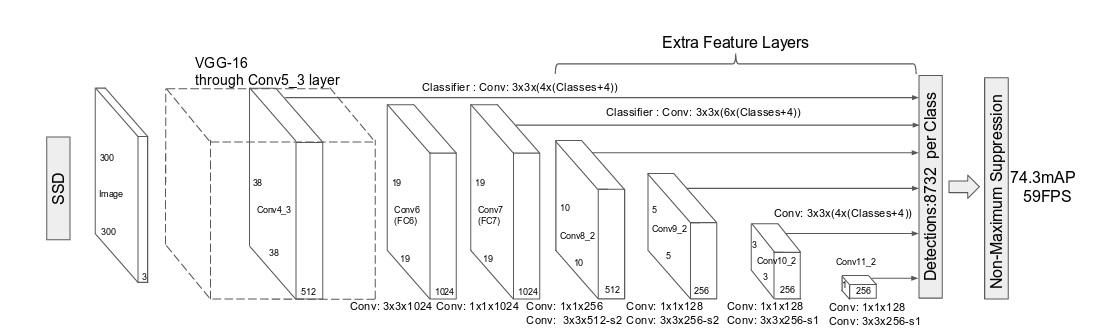
\includegraphics[width=1.1\textwidth]{figures/Diseno_global/ssd300.png}
   \caption{Red SSD}
	\label{fig.ssd_300}
\end{center}
\end{figure}

VGG-16  está formada por 16 capas, de las cuales 13 son capas convolucionales, 2 capas totalmente conectadas y una capa de softmax que se emplea para clasificar. En la Figura ~\ref{fig.vgg16} se puede ver cual es la arquitectura de la red VGG.

 \begin{figure}
\begin{center}
	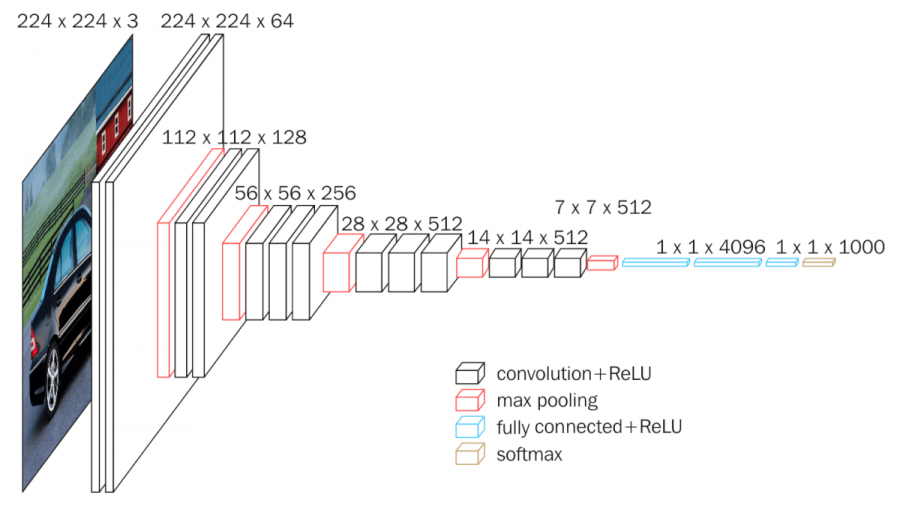
\includegraphics[width=0.8\textwidth]{figures/Diseno_global/vgg16.png}
   \caption{Red VGG-16}
	\label{fig.vgg16}
\end{center}
\end{figure}

\subsubsection{YOLO (Darknet)}

En este sistema se ha incluido \acrfull{yolo} debido a su gran éxito actualmente. \acrshort{yolo} ~\cite{yolo_article1} es otro enfoque para la detección de objetos. El trabajo previo a YOLO emplea clasificadores para realizar la detección. En esta aproximación, se enmarca la detección de objetos como un problema de regresión en \textit{bounding boxes} espacialmente separados y probabilidades de clase asociadas. En la evaluación, una red neuronal única predice \textit{bounding boxes} y probabilidades de clase directamente desde imágenes completas. Como todo el \textit{pipeline} de la detección es una red única, se puede optimizar la red de extremo a extremo directamente.

El sistema de \acrshort{yolo} divide la imagen de entrada en una cuadrícula SxS. Si el centro de un objeto cae en una celda de cuadrícula, esa celda de cuadrícula es responsable de detectar ese objeto. Cada celda de cuadrícula predice B \textit{bounding boxes} y las puntuaciones de confianza para esos \textit{bounding boxes}. Estas puntuaciones de confianza reflejan cómo está de seguro el modelo de que el \textit{bounding box} contiene un objeto y también cómo de preciso es el \textit{bounding box} que predice. Si no hay objeto en esa celda, las puntuaciones de confianza deben ser cero. De lo contrario, se espera que la puntuación de confianza sea igual al \textit{Intersection Over Union} (IOU) entre el \textit{bounding box} predicho y el \textit{ground truth}.

YOLO impone fuertes restricciones espaciales en las predicciones de los \textit{bounding boxes}, ya que cada celda de la cuadrícula solo predice dos \textit{bounding boxes} y solo puede tener una clase. Esta restricción espacial limita el número de objetos cercanos que nuestro modelo puede predecir. 

El modelo implementado es una red neuronal convolucional, donde ls capas convolucionales iniciales extraen características de la imagen, mientras que las capas \textit{fully connected} predicen las probabilidades y coordenadas de salida. La red tiene 24 capas convolucionales seguidas por 2 capas \textit{fully connected}. 

La arquitectura unificada de \acrshort{yolo} ~\ref{fig.yolov3} es extremadamente rápida, procesando imágenes en tiempo real a 45 frames por segundo. Una versión más pequeña de la red, Fast \acrshort{yolo}, procesa 155 frames por segundo, logrando duplicar el mAP (mean Average Precision) de otros detectores en tiempo real.

\begin{figure}
\begin{center}
	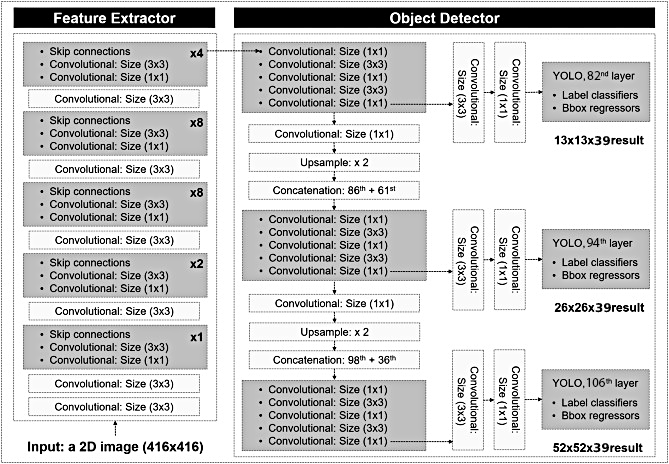
\includegraphics[width=0.9\textwidth]{figures/Diseno_global/yolov3.png}
   \caption{Arquitectura YOLO}
	\label{fig.yolov3}
\end{center}
\end{figure}

En comparación con los sistemas de detección más modernos, YOLO comete más errores de localización (especialmente con objetos pequeños), pero es menos probable que prediga falsos positivos en el fondo. Finalmente, \acrshort{yolo} aprende representaciones muy generales de objetos. Supera a otros métodos de detección, incluidos DPM y \acrshort{rcnn}, como en imágenes naturales y trabajos artísticos.

\subsubsection{Diseño Final}

En el diseño final de Smart-Traffic-Sensor se usa Darknet, pues es el framework con el que hemos obtenido mejores resultados. Todas las pruebas realizadas para llegar hasta este diseño quedan explicadas en el Capítulo ~\ref{cap.experimentos}.

El sistema del que partíamos (\textit{Traffic-Monitor} ~\cite{traffic_monitor_redo}) definía en la imagen una zona de entrada y otra de seguimiento. Esto puede verse en la Figura ~\ref{fig.zonas}.

\begin{figure}
\begin{center}
	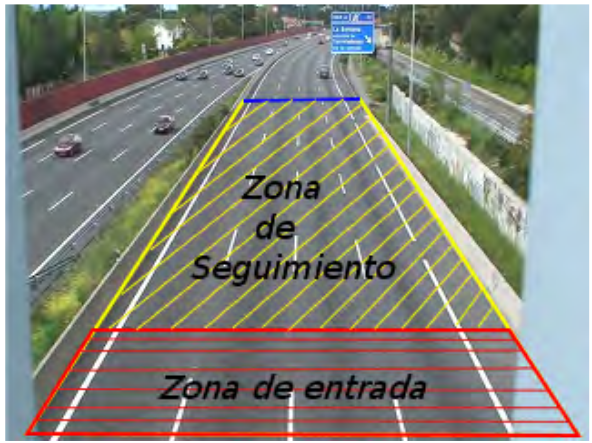
\includegraphics[width=0.7\textwidth]{figures/Diseno_global/zonas.png}
   \caption{Zonas de entrada y seguimiento}
	\label{fig.zonas}
\end{center}
\end{figure}

En la zona de entrada se realizan las detecciones y en la de seguimiento es donde se lleva a cabo la clasificación y el tracking de los vehículos.

Este concepto de separar zona de entrada y seguimiento va a perder relevancia en nuestro sistema, pues ya no va a ser necesario hacer esta distinción. Tendremos una única zona en la que se lleve a cabo la detección, la clasificación y el tracking. Vamos a continuar teniendo una zona marcada en la imagen para identificar en que parte de la carretera queremos centrar nuestras detecciones ( por si existiesen carriles de diferente sentido). A esta zona de detección , clasificación y seguimiento vamos a llamarle zona de evaluación. En la Figura ~\ref{fig.nueva_zona} se puede ver la zona  de evaluación.

\begin{figure}
\begin{center}
	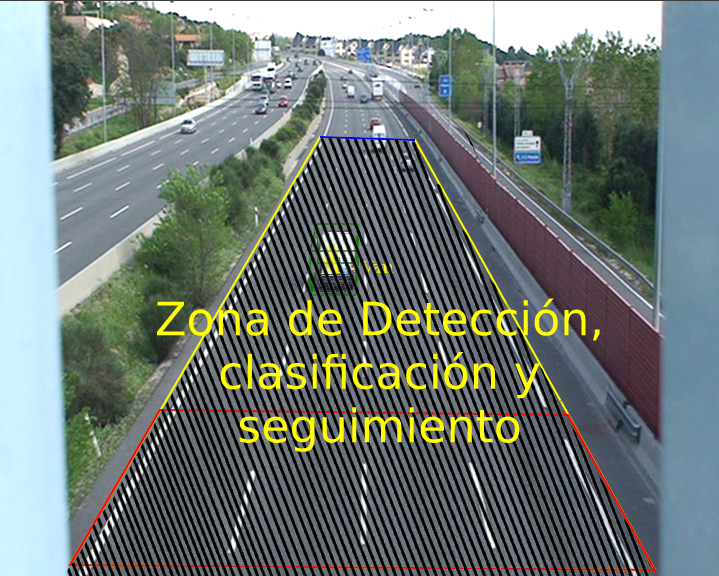
\includegraphics[width=0.7\textwidth]{figures/Diseno_global/nueva_zona.png}
   \caption{Zona Evaluación}
	\label{fig.nueva_zona}
\end{center}
\end{figure}

La detección y clasificación de los vehículos se realiza gracias al uso de Deep Learning. En este caso gracias al uso de Darknet (\acrshort{yolo}). En videos en carretera es muy probable que tengamos oclusiones y por supuesto vehículos que se vayan alejando, los cuales son bastante complejos de detectar. Para solventar esto nos hemos apoyado en \acrshort{klt}. Por tanto tenemos un sistema que complementa Deep Learning con KLT. 

Para tener un sistema lo más robusto posible se han tenido en cuenta varios detalles:

\begin{itemize}
    \item Dentro de la zona de evaluación tenemos dos zonas. En la
     Figura ~\ref{fig.zona_evaluacion} quedan identificadas esas dos zonas.
.    \begin{figure}
\begin{center}
	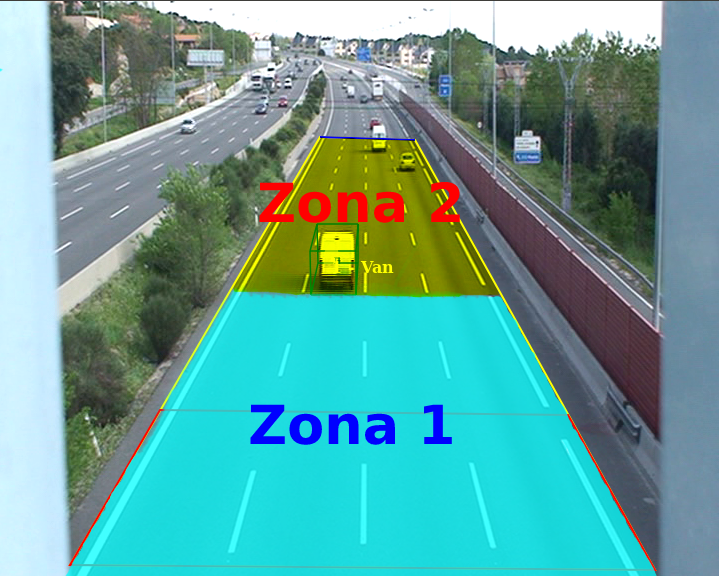
\includegraphics[width=0.7\textwidth]{figures/Diseno_global/zonas_evaluacion.png}
   \caption{Zonas de Evaluación}
	\label{fig.zona_evaluacion}
\end{center}
\end{figure}
    La zona 1 se corresponde con la mitad de la zona de evaluación por donde entran los vehículos. En esta zona es mas sencillo detectar y clasificar los vehículos pues tienen mayor tamaño. La zona 2 hace referencia a la mitad por la que salen los vehículos, la cual es más compleja, pues los vehículos tendrán menor tamaño.
    \item Un vehículo siempre va a entrar a la zona de evaluación por la parte de entrada. Nunca puede aparecer de repente. Por ello no puede aparecer ningún vehículo nuevo en el medio de la carretera, es decir nunca se podrá estimar que se ha detectado un vehículo nuevo en la zona 2.
    \item Si en la zona 1 un vehículo no es detectado durante 5 secuencias seguidas se dará por echo que ha sido un falso positivo y por tanto quedará descartado.
    \item Todo vehículo que se encuentre en la zona 2 se considerará que es un vehículo correcto. Si mediante Deep Learning no somos capaces de detectar dicho vehículo, emplearemos \acrshort{klt} para localizarlo. Es decir, nos apoyaremos en el seguimiento para realizar la detección.
\end{itemize}

Como \acrshort{klt} va asociado al seguimiento de objetos se explicará en la Sección ~\ref{sec.seguimiento}.


\subsection{Seguimiento de Vehículos}\label{sec.seguimiento}

Una vez tenemos los vehículos detectados y clasificados debemos realizar su seguimiento a lo largo de la carretera. Es decir, tenemos que asociar cada blob detectado a los blob anteriores de los que ya se llevaba un seguimiento. El algoritmo empleado para realizar este tracking está basado en la proximidad espacial.

La diferencia de píxeles en la imagen entre la posición de un vehículo en \textit{t-1} y en \textit{t} es muy pequeña. Por tanto se puede decir que el blob de un vehículo en \textit{t} cae en una zona muy cercana al blob de ese mismo vehículo en \textit{t-1}. Esto se tendrá en cuenta a la hora de realizar el seguimiento, ya que cuando busquemos un vehículo en \textit{t} deberíamos enncontrarlo en un radio circular pequeño alrededor de la posición de ese mismo vehículo en \textit{t-1}. 

El algoritmo que se plantea en cuanto a la proximidad espacial es el empleado por Redouane Kachach ~\cite{redo_tesis}. En él se estima el área donde debería localizarse un vehículo en función de su posición en \textit{t-1}. A medida que los vehículos vayan avanzando este área se irá actualizando.

Al principio el área se toma como un círculo pues no tenemos suficientes datos acerca de su orientación. Pero a medida que el vehículo avanza y tenemos suficiente información para conocer su orientación tomaremos el área como una elipse con centro en el centro del vehículo en \textit{t-1}. 

Consideraremos que tenemos suficiente información para estimar su orientación cuando tengamos 6 posiciones de un vehículo. Se empleará regresión lineal para calcular la orientación del vehículo basándonos en la posición que va tomando el vehículo a medida que va avanzando. 

La regresión lineal consiste en minimizar $\sum_{i}\rho(r_i)$ , donde $r_i$  es la  distancia  con  el  i-ésimo  punto  y $\rho(r_i)$ es una función de la distancia. $\rho(r_i)$ se puede calcular como:

\begin{equation}\label{ec.regresion_lineal}
   \rho(r_i) = 2(\sqrt{1 +\frac{r^2}{2}} - 1) 
\end{equation}

Una vez tenemos información acerca de la orientación definiremos el área de búsqueda como una elipse que tiene como centro el mismo que el vehículo en \textit{t-1} y dirección la calculada con la Fórmula ~\ref{ec.regresion_lineal}.

Los emparejamientos entre los vehículos detectados en el instante \textit{t} y los blob almacenados del instante \textit{t-1} se limitarán a los vehículos que caen dentro del área del círculo o la elipse que se obtiene en función de la posición del vehículo en el instante \textit{t-1}. En la Figura ~\ref{fig.area_vehiculo} se puede ver la evolución que sufre el área alrededor del vehículo a medida que avanza.

 \begin{figure}
\begin{center}
	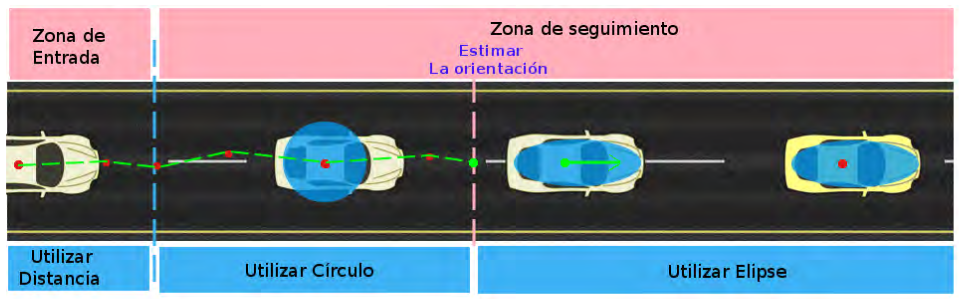
\includegraphics[width=0.9\textwidth]{figures/Diseno_global/areas_vehiculo.png}
   \caption{Evolución del área alrededor del vehículo}
	\label{fig.area_vehiculo}
\end{center}
\end{figure}


Estas elipses de definen como $C_{xc,yc,\omega}$, donde $\omega$ es la orientación y $(x_c, y_c)$ es el centro del vehículo. Además a la hora de describiir una elipse debemos conocer sus dos ejes. Estos parámetros se pueden ver en la Figura ~\ref{fig.elipse}.

 \begin{figure}
\begin{center}
    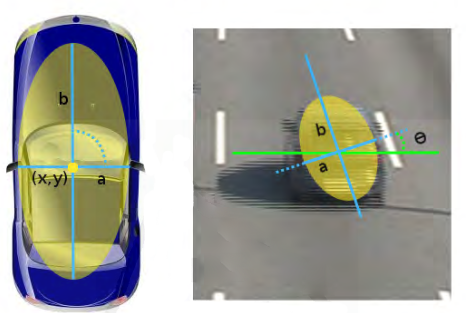
\includegraphics[width=0.7\textwidth]{figures/Diseno_global/elipse.png}
   \caption{Elipse asociada a los vehículos}
	\label{fig.elipse}
\end{center}
\end{figure}

Un blob 2D cuyo centro es $B(x,y)$ se encontrará dentro de la elipse  $C_{xc,yc,\omega}$ si se cumple:

\begin{equation}\label{ec.blob_elipse}
   C_{\omega} = \arctan(\frac{a_x}{a_y})
\end{equation}

\begin{equation} \scriptsize \label{ec.blob_elipse1}
   \left(\frac{cos(C_\omega)(B_x - C_{x_c}) + sin(C_\omega)(B_y - C_{y_c})}{a} \right)^2 + \left(\frac{cos(C_\omega)(B_y - C_{y_c}) - sin(C_\omega)(B_x - C_{x_c})}{b} \right)^2 \leq 1
\end{equation}

$a_x$ y $a_y$ son los componentes del vector de orientación. En la Figura ~\ref{fig.emparejamiento_blob} se puede ver como se realiza el tracking entre dos blob consecutivos. 

 \begin{figure}
\begin{center}
   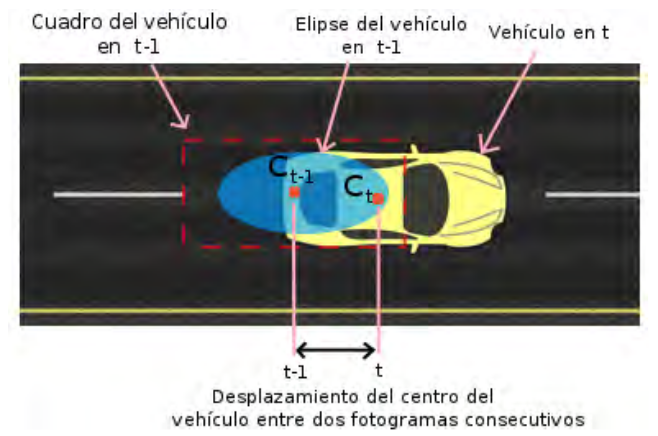
\includegraphics[width=0.7\textwidth]{figures/Diseno_global/emparejamiento_blob.png}
   \caption{Seguimiento con proximidad espacial}
	\label{fig.emparejamiento_blob}
\end{center}
\end{figure}

En resumen una detección deberá encontrarse dentro de un cierto área alrededor del blob detectado en \textit{t-1} para poder ser identificado como el mismo vehículo. Podría darse el caso de que dos vehículos cayeran en dicho área. Por ello es necesario tener en cuenta la distancia euclídea entre el centro del blob del instante \textit{t-1} y el centro de los blob en \textit{t} . Aquel blob del instante \textit{t} que se encuentre a menor distancia del blob del instante \textit{t-1} y por supuesto esté dentro del área alrededor del blob \textit{t-1} será considerado como el mismo vehículo que el de \textit{
t-1}. Es decir si esto se cumple el blob de \textit{t-1} y \textit{t} corresponden al  mismo vehículo pero en instantes consecutivos.

Como ya se ha mencionado en apartados anteriores si no se detacta un vehículo ya sea porque haya alguna oclusión o se encuentre muy lejos se empleará \acrshort{klt} que es muy robusto y se ha visto que funciona incluso ante oclusiones.

Para poder realizar \acrshort{klt} necesitamos conocer el centro de masas de los vehículos y sus características visuales. En función de los puntos característicos del vehículo en \textit{t-1} , \acrshort{klt} calculará el emparejamiento para cada punto característico y como resultado generará un nuevo conjunto de puntos correspondientes al vehículo en cuestión. Para llegar a conseguir un emparejamiento correcto el sistema se basa en votos. A cotinuación se va a explicar más en detalle \acrshort{klt}.

Jean-Yves Bouguet~\cite{klt_bouguet} hicieron una implementación de \acrshort{klt} en la cual aplicaban \acrshort{klt} de forma recursiva sobre una pirámide de imágenes. Este misma implementación es la que se ha empleado en este trabajo. 

Lukas Kanade es un método diferencial y local en el que se analiza la vecindad de cada píxel. En él se asume que el flujo óptico es constante en una vecindad, y se resuelve la ecuación del flujo
óptico para todos los píxeles en esta vecindad por el método de los mínimos cuadrados. Para el cálculo de los vectores de velocidad se emplea la siguiente fórmula:

\begin{equation}\label{klt_formula}
   \begin{bmatrix}u \\ v\end{bmatrix} = \begin{bmatrix}
            \sum_{i}I_{xi}^2 & \sum_{i}I_{xi}I_{yi} \\
            \sum_{i}I_{xi}I_{yi} &  \sum_{i}I_{yi}^2 \\
\end{bmatrix}^{-1} \begin{bmatrix}
-\sum_{i}I_{xi}I_{ti} \\
-\sum_{i}I_{yi}I_{ti} \\
\end{bmatrix}
\end{equation}
\\

El vector $(u,v)$ es el vector de desplazamiento del flujo óptico.
$I_x$ es la media del gradiente en x entre dos imágenes consecutivas, es decir, si $I(t)$ es la imagen del instante actual e $I(t+1)$ es la imagen en el instante siguiente, la $I_x$ de estos fotogramas es:

\begin{equation}
    I_x = \frac{I_x(t)+I_x(t+1)}{2}
\end{equation}

$I_x(t)$ es el gradiente en el eje x de la imagen $I(t)$ e $I_x(t+1)$ es el gradiente en $x$ de la imagen $I(t+1)$. $I_y$ es la media de los gradientes en $y$ de la imagen $I(t)$ e $I(t+1)$:

\begin{equation}
    I_y = \frac{I_y(t)+I_y(t+1)}{2}
\end{equation}

$I_t$ es la diferencia entre $I(t)$ suavizada e $I(t+1)$ suavizada:

\begin{equation}
   I_t = I'(t+1) - I'(t) 
\end{equation}

Tal y como se ha dicho \acrshort{klt} se aplica en forma de kernels de tamaño $\omega x \omega$ a lo largo de la imagen. El tamaño de los kernels debe ser definido en función de la cantidad de movimiento que tenga la imagen. Un valor de kernel pequeño será idóneo para evaluar desplazamientos pequeños de un punto. El uso de un tamaño grande de kernel aumenta el riesgo de obtener un error, pero hay en casos en los que el desplazamiento de un punto es muy grande y esto es necesario.

En la Figura ~\ref{fig.klt_piramidal} se puede ver como funciona \acrshort{klt} de forma piramidal.

 \begin{figure}
\begin{center}
	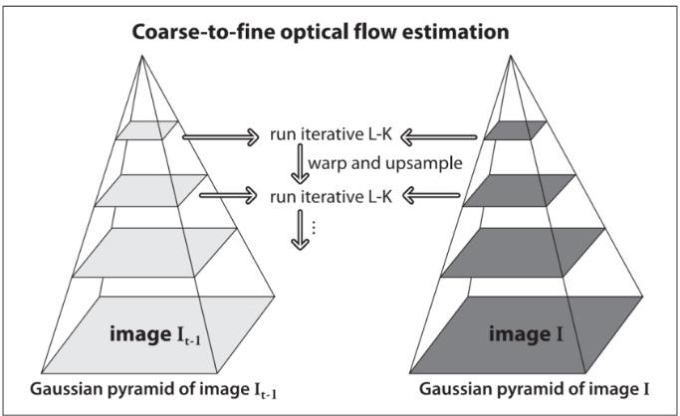
\includegraphics[width=0.7\textwidth]{figures/Diseno_global/klt_piramidal.png}
   \caption{\acrshort{klt} Piramidal}
	\label{fig.klt_piramidal}
\end{center}
\end{figure}

Gracias al empleo de \acrshort{klt} piramidal se pueden estimar grandes desplazamientos con un tamaño de ventana muy pequeño.

En resumen el seguimiento se realiza mediante la proximidad espacial pero se hará uso de \acrshort{klt} en casos problemáticos, haciendo asi más robusto nuestro sistema. \acrshort{klt} se calculará en todas las secuencias para ir actualizando los puntos característicos.

\subsection{Resumen General del Sistema}

Smart-Traffic-Sensor ha sido diseñado para llevar a cabo la monitorización de vehículos.  Esta monitorizacion consta de tres elementos principales:

\begin{itemize}
    \item Detección de vehículos
    \item Clasificación de vehículos
    \item Seguimiento de vehículos
\end{itemize}

Las detecciones y la clasificación van de la mano, pues se realizan con Deep Learning. En concreto con una red de \acrshort{yolo}. El seguimiento se centra en la proximidad espacial, y si esta falla se utliza \acrshort{klt}. A todos los blob detectados se les realizará un seguimiento a lo largo del tiempo.

En cuanto a las detecciones y la clasificación hay que tener en cuenta que no pueden aparecer vehículos nuevos en medio de la imagen, por tanto si eto sucede se considerará un falso positivo y se descartará. Otro aspecto que hay que tener en cuenta es que se podría dar una detección errónea, por ello si durante 5 secuencias seguidas un vehículo no ha sido detectado se considerará como que era un falso positivo y se dejará de hacer su seguimiento.

El seguimiento se centra en asociar las detecciones actuales con los blobs almacenados del instante anterior. En el seguimiento se tendrán ciertos aspectos en cuenta:

\begin{itemize}
    \item Si un blob llega al final de la zona de evaluación se eliminará del seguimiento.
    \item Se recorrerán los blob del instate \textit{t-1} almacenados con el fin de emparejarlos con los blob detectados en el instante \textit{t}. Este emparejamiento se establecerá entre los blob \textit{t} y \textit{t-1} que tengan menor distancia euclídea entre sus centros.
    \item Si el blob \textit{t} asociado al blob \textit{t-1} no cae dentro del área circular o elíptica que se genera alrededor del centro del blob \textit{t-1} no quedará emparejado a este. 
    \item Si mediante proximidad espacial no somos capaces de emparejar un blob \textit{t-1} emplearemos \acrshort{klt}.
\end{itemize}

\section{Estimación de la Velocidad}

Smart-Traffic-Sensor tiene opciones para configurar la cámara, es decir para realizar su calibración. Al tener información de la cámara empleada tendremos información 3D de la imagen. Es decir podemos realizar una proyección al mundo 3D de nuestros puntos en la imagen.

Para calcular la velocidad solo necesitamos conocer la distancia que ha recorrido el vehículo y el tiempo que ha tardado en hacerlo. Disponemos de una zona de evaluación por la cual discurren los vehículos, por tanto podemos saber cuanta distancia recorre por dicha zona de evaluación y el tiempo que tarda en hacerlo. Para calcular la distancia tenemos que calcular la posición 3D de los vehículos y con ella hacer su diferencia.


